% !TEX root =  ../main.tex

\section{Model}



\begin{figure*}
\centering
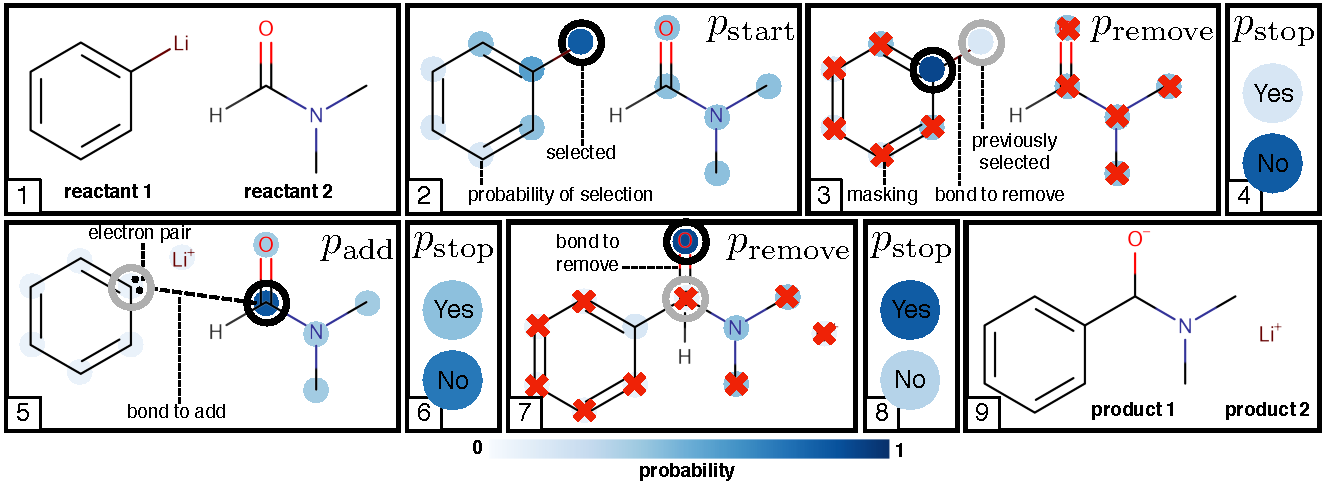
\includegraphics[width=\textwidth]{reaction_model_blue}
\caption{A visualization of the actions taken by the model to sequentially perform a simple reaction.}
\label{fig:reaction_model}
\end{figure*}



In this section we define a probabilistic model that describes the flow of movement of electrons that define an elementary heterolytic reaction.
We represent a set of molecules as a set of graphs $\moleculeSet$, with atoms $\Ac$ as vertices and bonds $\Bc$ as edges;
each connected component of the graph defines an individual molecule.
We can associate an ordering over all the atoms in all the molecules in the set using an {\em atom map} number,
an integer label assigned to each non-hydrogen atom in both the reactants and the products which 
both permits easy matching between atoms before and after the reaction, and
%\footnote{In the USPTO dataset, all reactions have been ``atom mapped'', which means that integer labels have been assigned to each non-hydrogen atom in both the reactants and the products.}. 
gives us a consistent way to index particular atoms.
Each atom $v \in \Ac$ includes a set of features, which are described in the supplementary material.
Input molecules into the model are first put in a Kekul\'e form, a process which makes explicit the location of single and double bonds in aromatic structures;
each bond $b \in \Bc$ is either a single, double, or triple bond.


Given an initial set of reactant molecules $\moleculeSet_0$ and a set of reagent molecules $\moleculeSet_r$, 
our model defines a conditional distribution over a sequence of atoms $\electronPath_{0:T} = (a_0, a_1, \ldots, a_T)$,
which fully characterizes the electron path.
\improvement[]{maybe instead $\electronPath$ goes up to $T-1$ and $\moleculeSet$ goes up to $T$? then both are length $T$}
This electron path in turn deterministically defines both a final product $\moleculeSet_{T+1}$, 
denoting the outcome of the reaction,
as well as a sequence of intermediate products $\moleculeSet_t$, for $t = 1,\dots,T$,
which correspond to the state of the graph after the first $t$ steps in the subsequence $\electronPath_{0:t} = (a_0, \dots, a_t)$ are applied to the initial $\moleculeSet_0$.


We propose to learn a parameterized distribution $p_\theta( \electronPath_{0:T} \mid \moleculeSet_0, \moleculeSet_r)$ over electron movements. 
We begin by describing the generative process %(i.e., the forward pass) 
of $p_\theta$, and then describe how to train the model parameters.


\subsection{Generative process}

The joint probability of an electron path can be factorized into a product of distributions
defining the probability $p(a_0 \mid \initialAndReactants)$ of the initial state $a_0$ given the reactants and reagents, 
the conditional probability $p(a_t \mid a_{t-1}, \moleculeSet_t, t)$ \todo[]{maybe somehow refer to "bond type" instead of $t$?} of next state $a_t$ given the intermediate products $\moleculeSet_t$ for $t > 0$,
and the probability $p(s_t \mid \moleculeSet_t)$ that the reaction terminates with final product $\moleculeSet_{t}$.

%The distribution over electron paths can be factorized as follows:
%%\begin{align}
%%p_\theta(\electronPath \mid \moleculeSet_0) = p_\theta(s_{0}' \mid \moleculeSet_0) p_\theta(a_{0} \mid \moleculeSet_0) \prod_{t=1}^{T-1} \left( p_\theta(a_{t} \mid a_{t-1}, \Mc_{t-1} ) p_\theta(s_{0}' \mid \moleculeSet_0) \right) p_\theta(a_{T} \mid a_{T}, \Mc_{T-1} ) p_\theta(s_{T} \mid \moleculeSet_T) \nonumber
%%\end{align}
%
%\begin{align*}
%p(\electronPath_{0:T} \mid \initialAndReactants) = &
% \quad 
% p(s_0' \mid \initialAndReactants)
% p(a_0 \mid \initialAndReactants)
% \prod_{t=1}^{T} \Big[ 
% 	p(s_t' \mid \initialAndReactants, \electronPath_{0:t-1})
% 	p(a_t \mid \initialAndReactants, \electronPath_{0:t-1} ) 
% \Big] \\
% & \times p(s_{T+1} \mid  \initialAndReactants, \electronPath_{0:T} )
%\end{align*}

%\improvement[]{this part a bit messy}
%Where $p(s_{t})$ is the probability of stopping the path before picking the $t^{\text{th}}$ action, $p(s_{t}')$ of continuing.


In practice we assume that the probability of an action depends only on (i) the intermediate molecule formed by the action path up to that point, (ii) the previous action taken (indicating where the free pair of electrons are) and (iii) the point of time through the path, indicating whether we are on an add or remove bond step. 
We further make the simplifying assumption that the stop probability and the actions after $a_0$ do not depend on the reagents. This leads to a parameterized model with dependency structure:
\begin{align}
p_\theta(\electronPath_{0:T} \mid \moleculeSet_0, \moleculeSet_r) 
&=
	   p_\theta(s'_0 \mid \moleculeSet_0)
       p_\theta(a_0 \mid \moleculeSet_0, \moleculeSet_r)\\ \nonumber &\quad \times
	\left[\prod_{t=1}^{T}
		p_\theta(s_{t}' \mid \moleculeSet_{t})
		p_\theta(a_t \mid \moleculeSet_{t}, a_{t-1}, t)
	\right]
	p_\theta(s_{T+1} \mid \moleculeSet_{T+1})
	,
\label{eq:jointprob}
\end{align}
where we have defined $p(s'_t \mid \moleculeSet_t) \equiv 1 - p(s_t \mid \moleculeSet_t)$ to be the probability of {\em continuing} a reaction given the current molecule set $\moleculeSet_t$.
%
%
%%% THIS IS THE PREVIOUS VERSION:
%\begin{align*}
%p_\theta(\electronPath_{0:T} \mid \moleculeSet_0, \moleculeSet_r) = &
% \quad \continueProb{0}{0}
%       p(a_0 \mid \moleculeSet_0, \moleculeSet_r)
%       p(a_1 \mid \moleculeSet_0, a_0) \\
%       & \times \prod_{t=2}^{T} \Big[
%              \continueProb{t}{\electronPath_{0:t-1}}
%              \actionProb{t}
%       \Big] \\
%       & \times p(s_{T+1} \mid \moleculeSet_{\electronPath_{0:T}})
%\end{align*}
%
Note that you cannot stop after one action, as you have to pick up a complete electron pair;
however, it is possible to stop prior to selecting a first atom $a_0$, indicating that no reaction would take place.
Given any particular selected atom $a_t$ which extends the reaction path, we can deterministically update the previous molecular graph $\moleculeSet_{t}$ to produce the next set of (intermediate) products $\moleculeSet_{t+1}$.

If the three reaction assumptions stated in the previous section hold, then, as stated earlier, there are two types of electron movements that alternate: 
(1) movement that \emph{removes an existing bond}, and 
(2) movement that \emph{adds a new bond}. 
We can generalize assumption 3 by defining that atoms with free electrons have a self-bond. 
Thus, all reactions start by first selecting an atom, removing a bond (between two different atoms, or a self-bond), and then alternately adding and removing bond;
we can determine whether a particular step is an add step or remove step by inspecting $t$.
Note that $\moleculeSet_1 = \moleculeSet_0$, as the initial action of selecting $a_0$ does not remove or form any bonds\todo{maybe put this somewhere else}.

Each of the conditional probabilities in Eq.~\eqref{eq:jointprob} is parameterized by a neural network:
for each stage the network takes the current intermediate product graph, 
along with the previous action and the reagents if relevant, 
to compute a probability distribution over next possible actions (i.e., selecting a particular atom, or stopping).
These structure of these networks will be described in the following section and more detailed information on the architectures is given in the supplementary material.

Figure~\ref{fig:reaction_model} shows a simple example reaction, which demonstrates all the critical features of the model.
The first subfigure shows two reactants, which we assume will react (i.e.\ $s_0' = 1$).
Subsequent subfigures show the network picking an initial atom to begin the electron path,
and then iteratively selecting atoms for removing and adding bonds, potentially stopping after each action.
Masking at each add and remove step can reduce the total number of possibilities: 
for example, it is not possible to remove a bond which does not exist in the graph $\moleculeSet_t$.
\todo[]{walk through figure. do we want to that HERE, or in the caption? or elsewhere?}

\subsection{Computing atom and molecule features}


We are left now with describing how we define our conditional distributions for continuing, $p_\theta(s'_t \mid \moleculeSet_t)$, picking the initial action, $p_\theta(a_0 \mid \initialAndReactants)$, and picking subsequent actions, $p_\theta(a_t \mid a_{t-1}, \moleculeSet_t, t)$.
However, before describing these modules we need to describe how we compute node embeddings and graph embeddings as these  are  essential to each.

Node embeddings are representations of all the atoms (vertices) in all the molecules present in $\moleculeSet_t$.
 We denote them by the matrix $\nodeEmbeddings{\moleculeSet_t} \subseteq \Rc^{|\Ac|\times d}$.
Each row contains a $d$-dimensional embedding of an atom (vertex).
A natural ordering for the rows are  the corresponding atoms' atom-mapped numbers.
We define the function $\fEmbed$ to take in a set of graphs representing each molecule and compute these node embeddings.
 
In general $\fEmbed$ could be any deep graph model that uses the graph structure of $\Mc_t$ to get graph-isomorphic node features, usually via message-passing techniques \citep{gilmer2017neural}. 
We choose to use Gated Graph Neural Network (GGNN) message functions \citep{li2016gated}.

It is also useful to be able to calculate graph embeddings, $\graphEmbeddings$, which are vectors that represent groups of nodes belonging to one or more graphs.
 We define the function that takes node features belonging to one or more graphs, and calculates their graph embedding by $\fEmbedGraphs$.
These are similar to the readout functions used for regressing on graphs detailed in \citep[Eq. 3]{gilmer2017neural} and the graph embeddings described in \citet[\S B.1]{li2018learning}. \todo[]{check ref the correct parts of these other papers.}


More specifically $\fEmbedGraphs$ consists of three functions, $\fui$, $\fuj$ and $\fuk$, which could be any MLP but in practice we use linear layers for.
 There are two stages. 
In stage (i) similar to \citet[\S B.1]{li2018learning} we form an embedding of one or more graphs (with vertices $\Ac'$), by performing a gated sum over the node features:
\begin{align*}
	\graphEmbeddings = \sum_{v \in \Ac'} \left[ \mbox{sigmoid}(\fui(\Hb_{\Ac,v})) \cdot \fuj(\Hb_{\Ac,v}) \right]
\end{align*}
More specifically, the function $\fui$ is used to decide how much that node should contribute towards the embedding and $\fuj$ projects the node embedding up to a higher dimensional space, which like \citet[\S B.1]{li2018learning}, we choose to be double the dimension of the node features.
Having formed this embedding of the graphs, we project this down to a lower dimensional space, which is done by function $\fuk$. 
Again we use a single linear layer for this function.


\subsection{Computing our probabilities over actions}

Having described how we compute node and graph embeddings we are now ready to describe each of our action modules. We start with $p_\theta(s'_t \mid \moleculeSet_t)$, which is the probability of continuing given the set of intermediate products at time $t$. This probability is computed as a graph embedding down to one dimension followed by a sigmoid function: $p_\theta(s'_t \mid \moleculeSet_t) = \sigma(\fEmbedGraphs_{\textrm{stop}}(\nodeEmbeddings{\moleculeSet_t}))$.


This leaves us with describing the form of the initial action, $p_\theta(a_0 \mid \initialAndReactants)$, and picking subsequent actions, $p_\theta(a_t \mid a_{t-1} \moleculeSet_t, t)$, modules.
 The second of these can be broken down into two parameterized functions
$p_\theta^\textrm{remove}(a_t \mid a_{t-1}, \moleculeSet_t)$ for the remove bond step, taken when $t$ is odd, and $p_\theta^\textrm{add}(a_t \mid \moleculeSet_t, a_{t-1})$ for the add bond step, taken when $t$ is even. 
 Each of these three parameterized conditional probability distributions for the {\em initial}, {\em add} and {\em remove} steps have similar forms, and produce a probability vectors over actions as their output. 
 
 Each of these modules start by computing  a single value for each node, so for the initial step we have 
 $\actionLogits_{\textrm{initial}, v} = \fum^\textrm{intial}(\nodeEmbeddings{\moleculeSet_t,v}, \contextVect)$ where $\fum$ is a NN and $\contextVect$ is a context vector. The expressions are similar for the add and remove modules, however with different NNs used for the respective $\fum$ functions.
 Moreover, they also differ in the context vectors, $\contextVect$, which they use; for the add, $p_\theta^\textrm{add}(a_t \mid \moleculeSet_t, t)$, and remove steps, $p_\theta^\textrm{remove}(a_t \mid \moleculeSet_t, t)$, this context vector is the node embedding of the previous action, $\nodeEmbeddings{\moleculeSet_t, a_{t-1}}$. 
 For the initial step, this context vector $\contextVect$ if computed by summing the graph embeddings for each reagent, computed using the embedding function $\fEmbedGraphs_r$.

Finally, each of the modules compute the probability vector over actions. So again starting with the initial step we have 
$p_\theta(a_0 \mid \initialAndReactants) \propto \bm{\beta_\textrm{initial}} \odot \mbox{softmax}(\bm{\actionLogits_{\textrm{initial}}})$, 
with again similar terms for the add and remove steps.  
The $\bm{\beta}$ term is a binary vector, that allows us to mask out specific actions. The value of this differs for the {\em initial}, {\em add} and {\em remove} steps. 
For the initial step any action (or atom) can be picked and so this is 1 everywhere. For the remove step, $\bm{\beta_\textrm{remove}}$ masks out bonds that do not currently exist (although self bonds are allowed in the first step).
For the add step, $\bm{\beta_\textrm{add}}$ only masks out the previous action.



\paragraph{Training}
We can learn the parameters $\theta$ of all the parameterized functions, by maximizing the likelihood of the true path $\log p_\theta(\electronPath_{0:T} \mid \moleculeSet_0, \moleculeSet_r)$.
%\begin{align*}
%%  \min_{\fModules}
%\min_{\theta}
%    & - \log \continueProb{0}{0} - \log p(a_0 \mid \moleculeSet_0, \moleculeSet_r)  - \log p(a_1 \mid \moleculeSet_0, a^*_0) \\
%	& - \sum_{t=2}^{T} \log \Big[ \continueProb{t}{\electronPath_{0:t-1}^*} \actionProb[*]{t} \Big] \\
%    & - \log p(s_{T+1} \mid \moleculeSet_{\electronPath_{0:T}^*})
%\end{align*}
This is evaluated by using a known true electron path $a_t^\star$ and intermediate products $\moleculeSet_t^\star$ extracted from training data,
rather than on simulated values. 
This allows us to train on all stages of the reaction at once.

\paragraph{Sampling}
Once trained we can sample chemically-valid paths from our model using beam search.  This is procedure is described in \todo[]{briefly describe beam search}. 



